\newpage


\section{Case Studies}
\label{sec:case-studies}

While the handcrafted NNs yielded relatively acceptable results we ask ourselves: how do other, well known,
model perform with such a trivial task? \\To answer this question two "case studies" were selected: Xception and VGG16.

\subsection{Xception}
\label{subsec:xception}

The Xception\cite{chollet2017xception} model was developed by Google and is an evolution of the Inception model presented
during the ImageNet Recognition Challenge of 2012, where AlexNet won.

In its latest definition Xception goes for a lower count of parameters of the model but, compared to Inception-v3
the difference is not extraordinary being only 1M less. What makes the model special is that uses depthwise separable
convolutions throughout the network\cite{understandingdeepwise}. % todo valuta se toglierlo
\begin{figure}[h]
    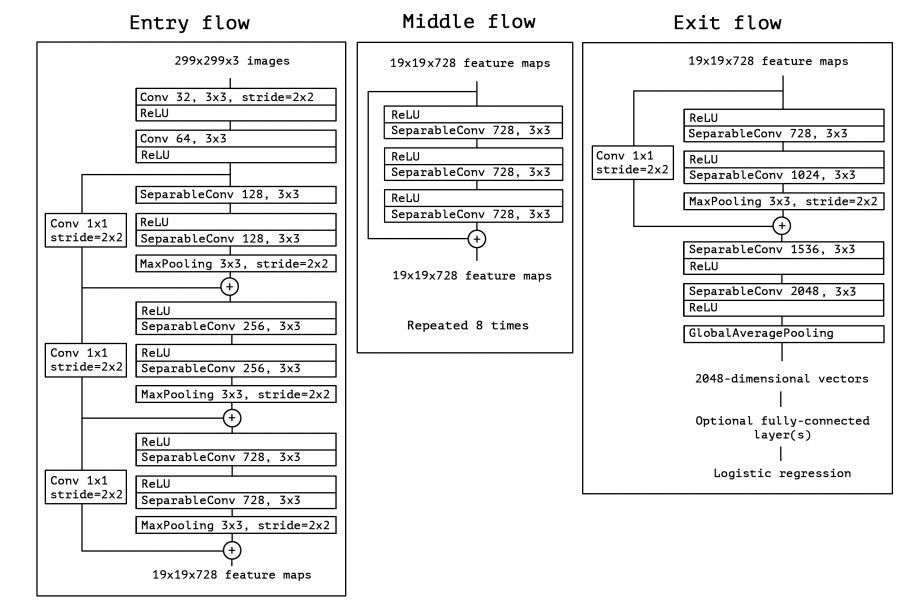
\includegraphics[scale=0.4]{imgs/xception-arch}
    \caption{
        Xception is made of a total of 71 layers.\\
        \textit{Image by the author of the original paper Francois Chollet\cite{chollet2017xception}}
    % todo ref

    }\label{fig:figure}
\end{figure}

\subsubsection{Xception applied to Muffin vs Chihuahuas}
\label{subsubsec:xception}

To measure the performance of Xception on the Muffin vs Chihuahuas task we first see the pretrained model in action
to later fine tune it on our dataset.

\paragraph{Pretrained Model} The pretrained model used for the evaluations has its trained on the
\textit{Imagenet} dataset. The dataset does not provide a label "muffin" so it was mapped to "bakery"(415) which
for our intent is close enough.

Predictions might not include either bakery or chihuahua as there are other classes, in this case we consider them as misclassifications.
% todo imggine risultati


\paragraph{Fine-tuned Model}
In order to fine tune the model and work with desirable results we have to define a new model that wraps around Xception.
The model has to use the pre-processing on data used by Xception as requested by the keras documentation. It is also
necessary to output a single prediction value instead of the previous top-k elements.

During the training process, which often takes very little time,  we freeze the network to not destroy the information
already built by the previous training process and only work up on the last layer of the \textit{Xception}.
%immagine modello
\begin{figure}[h]

        \centering
        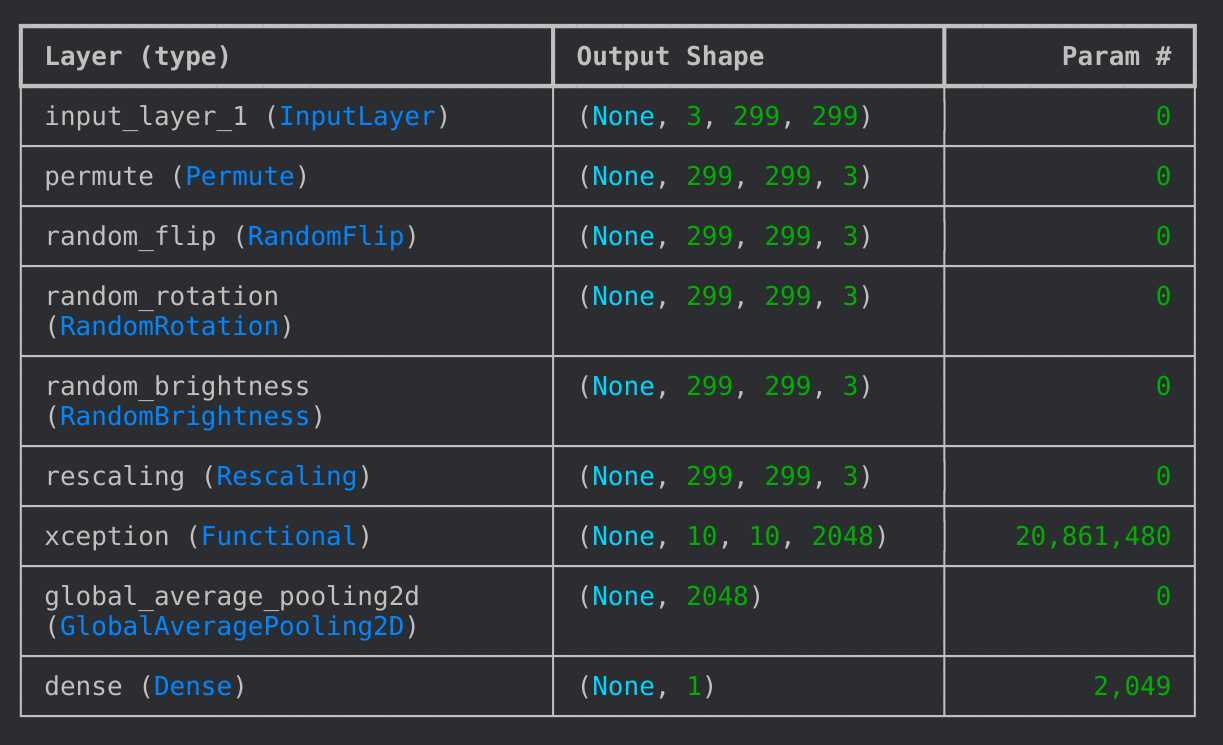
\includegraphics[scale=0.2]{/home/jacopo/PycharmProjects/muffin-stat-project/report/imgs/struct_xception_custom}
    \caption{
        Before calling \textit{Xception} the model preprocesses the data with the same augmentation procedure we defined for the other
        networks of the project. It then also rescales the images to meet the requirement for \textit{Xception}.
        At the top of the model we have now a single dense neuron layer that will return the classification output.
    }\label{fig:figurexception}
\end{figure}
% todo results
% immagine k fold



\subsubsection{Vgg16}
Developed by Visual Geometry Group (VGG) at the University of Oxford the VGG-16\cite{simonyan2015deep} is a deep CNN model that
was proposed for the ImageNet Large Scale Visual Recognition Challenge (ILSVRC) in 2014 where it achieved top results in object detection and image classification.

\begin{figure}[h]
    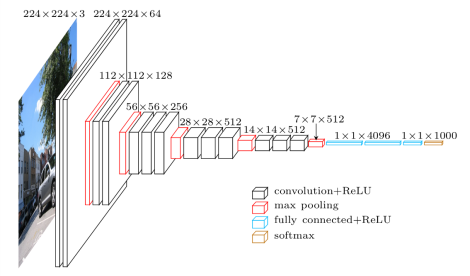
\includegraphics[scale=0.7]{imgs/vgg_arch}
    \caption{
        The VGG-16 model is characterized by 13 convolutionakl layers among which at times a max pooling layer has been placed.
        After those layers the network is closed by 3 fully connected layers with a final softmax classifier.
        \textit{Image by Davi Frossari (https://www.cs.toronto.edu/~frossard/about/)}
    }\label{fig:vgg16}
\end{figure}

Compared to Xception this model has more parameters

\subsubsection{VGG-16 applied to Muffin vs Chihuahuas}
The ideas we applied on Xception and the general methodology (\ref{subsubsec:xception}) are analogous to the ones
applied to \textit{VGG-16}.

\begin{figure}[h]

    \centering
    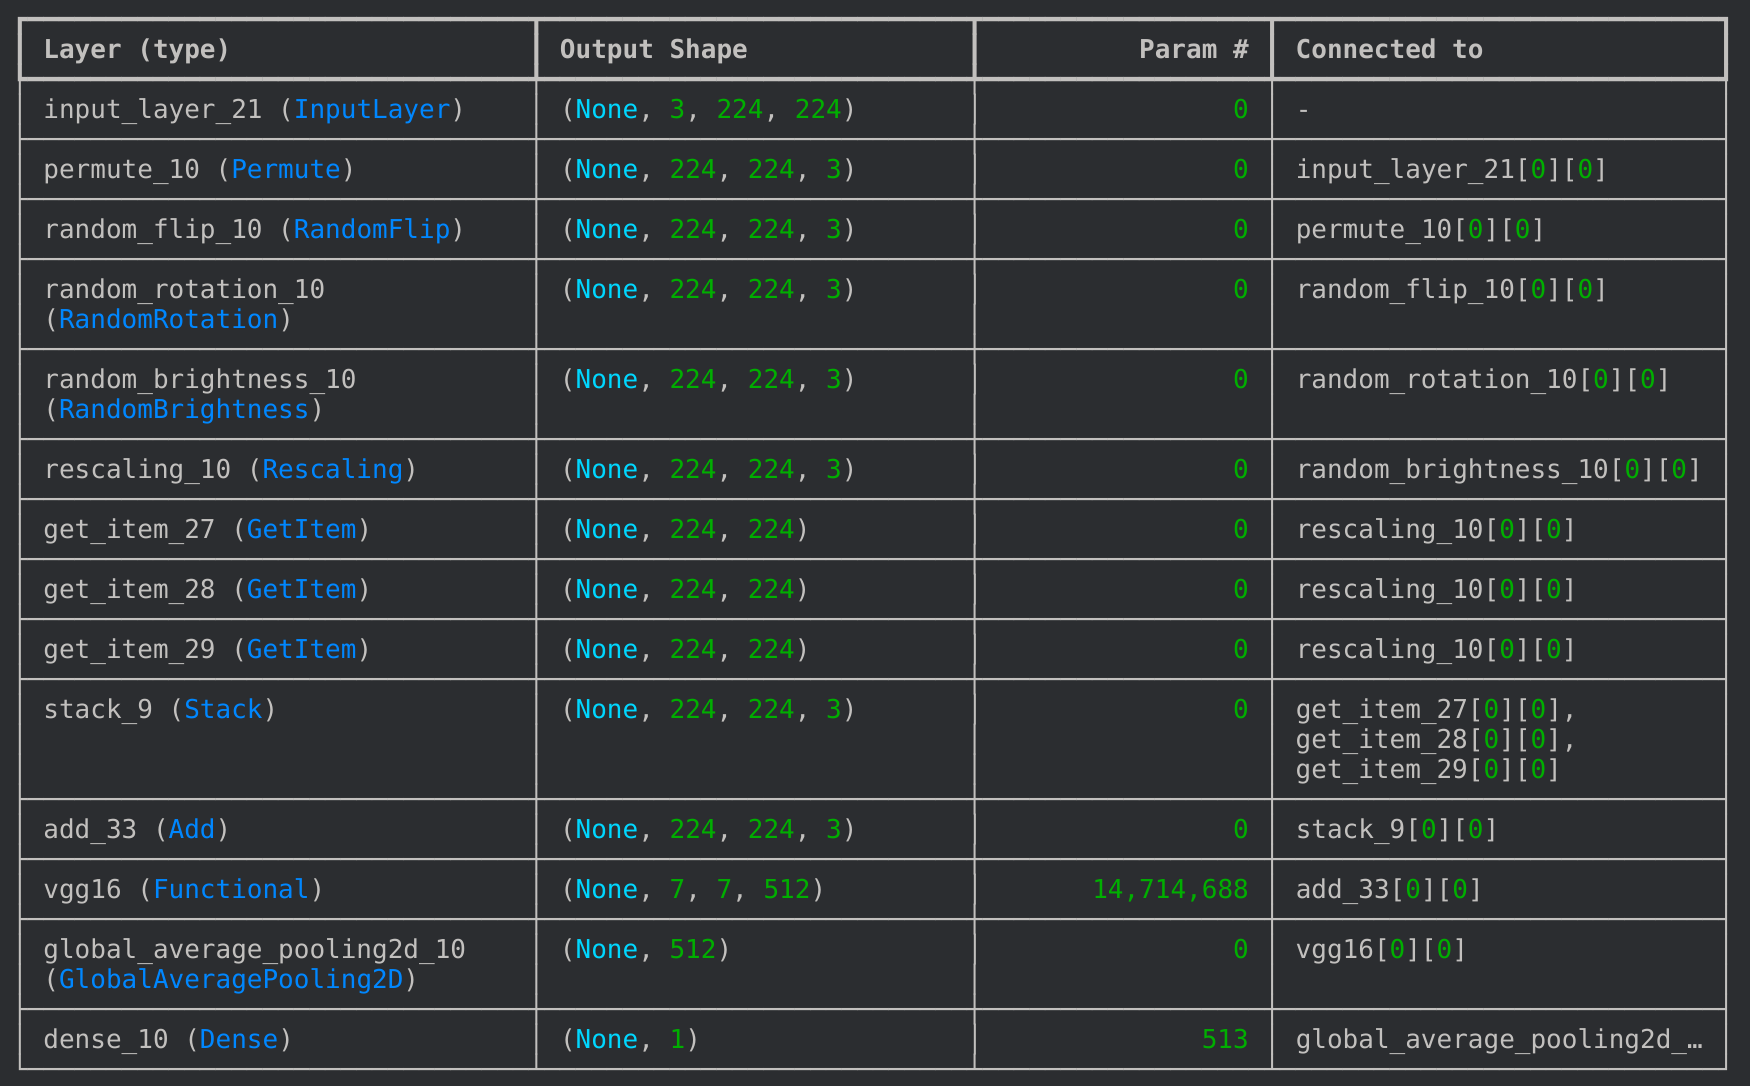
\includegraphics[scale=0.2]{/home/jacopo/PycharmProjects/muffin-stat-project/report/imgs/vgg-16-custom-structure}
    \caption{
        The structure is very similar same to \textit{Xception} with few differences being the \textit{Functional} model
        and the specialized pre-processing layers.
    }\label{fig:figurevgg16}
\end{figure}

\paragraph{Pretrained Model}
% todo results
\paragraph{Fine-tuned Model}
% todo results